%
% Master thesis template for Ghent University (2018)
%
%
%  !!!!!!!!!!!!!!!!!!!!!!!!!!!!!!!!!!!!!!!!!!!!!!!!!!!!!!!!!!!!
%  !!  MAKE SURE TO SET lualatex OR xelatex AS LATEX ENGINE  !!
%  !!!!!!!!!!!!!!!!!!!!!!!!!!!!!!!!!!!!!!!!!!!!!!!!!!!!!!!!!!!!
%  !! For overleaf:                                          !!
%  !!     1. click gear icon in top right                    !!
%  !!     2. select `lualatex` in "latex engine"             !!
%  !!     3. click "save project settings"                   !!
%  !!                                                        !!
%  !!!!!!!!!!!!!!!!!!!!!!!!!!!!!!!!!!!!!!!!!!!!!!!!!!!!!!!!!!!!
%
%
%  History
%    2014         Doctoral Thesis of Bruno Volckaert
%    2017         Adapted to master thesis by Jerico Moeyersons
%    2018         Cleanup by Merlijn Sebrechts
%
%  Latest version
%    https://github.com/galgalesh/masterproef-template
%
\documentclass[11pt,a4paper,twoside, openany]{book}
\usepackage[a4paper,includeheadfoot,margin=2.50cm]{geometry}

\setlength{\parindent}{0cm}           % indent of the first sentence of a paragraph
\setlength{\parskip}{1em}             % space between paragraphs
\renewcommand{\baselinestretch}{1.2}  % stretch horizontal space between everything

\usepackage{graphicx}
\graphicspath{{images/}}
\usepackage{pdfpages}
\usepackage{enumitem}
\usepackage{float}
\usepackage{caption}
\usepackage{subcaption}
\usepackage[toc,page]{appendix}

\usepackage{minted}                                    % for modern code highlighting
\newenvironment{code}{\captionsetup{type=listing}}{}   % To get multiline code fragments working: https://tex.stackexchange.com/a/53540/72273

\PassOptionsToPackage{hyphens}{url}
\usepackage{hyperref}
\usepackage{url}

\usepackage{quotchap}              % For the fancy quotes next to the chapter titles

\usepackage[numbers]{natbib}       % For bibliography; use numeric citations
\bibliographystyle{IEEEtran}
\usepackage[nottoc]{tocbibind}     % Put Bibliography in ToC

%
% Defines \checkmark to draw a checkmark
%
\usepackage{tikz}
\def\checkmark{\tikz\fill[scale=0.4](0,.35) -- (.25,0) -- (1,.7) -- (.25,.15) -- cycle;}

%
% For tables
%
\usepackage{booktabs}
\usepackage{array}
\usepackage{ragged2e}  % for '\RaggedRight' macro (allows hyphenation)
\newcolumntype{L}[1]{>{\raggedright\let\newline\\\arraybackslash\hspace{0pt}}m{#1}}
\newcolumntype{C}[1]{>{\centering\let\newline\\\arraybackslash\hspace{0pt}}m{#1}}
\newcolumntype{R}[1]{>{\raggedleft\let\newline\\\arraybackslash\hspace{0pt}}m{#1}}

%
% Support for splitting Dutch words correctly
%
\usepackage{polyglossia}
\setdefaultlanguage[babelshorthands=true]{dutch}

% Manually specify additional hypnations for words
%
% Translated strings. If these aren't set, the English words are used.
%
\addto\captionsenglish{%
  \renewcommand{\contentsname}%
    {Inhoudsopgave}%
}
\renewcommand\appendixtocname{Bijlagen}
\renewcommand\appendixpagename{Bijlagen}
\renewcommand{\listoflistingscaption}{Lijst van listings}

%
% Set the title and your name
%
\title{de titel}
\author{de auteur}

%
%  END OF HEADER
%  The actual latex document content starts here.
%
\begin{document}
%download het voorblad van plato
\includepdf{voorblad.pdf}             % Front matter
\newpage\thispagestyle{empty}\mbox{}  % White page
\thispagestyle{empty}    % Don't show page number

\begin{center}
\textbf{Dankwoord}
\end{center}

Vul aan          % Word of thanks
\newpage\thispagestyle{empty}\mbox{}  % White page
%om het extended abstract te schrijven kan je de IEEE conference proceedings template gebruiken. Die staat ook op Overleaf: https://www.overleaf.com/latex/templates/ieee-conference-template/grfzhhncsfqn. Voeg dit toe als .pdf
\includepdf[pages={-}]{abstract.pdf}  % Extended Abstract
\tableofcontents                      % Table of Contents
\listoffigures                        % List of figures
\listoftables                         % List of tables
\listoflistings                       % List of listings (code fragments)

%
% Include the main chapters of the thesis below
%
\begin{savequote}[0.55\linewidth]
	``If you think you've seen this movie before, //vul aan''
	\qauthor{\textasciitilde David Linthicum, author of Cloud Computing and SOA Convergence in Your Enterprise: A Step-by-Step Guide}
\end{savequote}

\chapter*{Inleiding}
\addcontentsline{toc}{chapter}{Inleiding}  
\label{chap:intro}

Vul aan
\section*{sectie titel}
\addcontentsline{toc}{section}{sectie title}  
\label{sec:what_is_cloud_computing}
Voorbeeld figuur

\begin{figure}
	\centering
	\begin{subfigure}{\textwidth}
		\centering
		\centerline{
			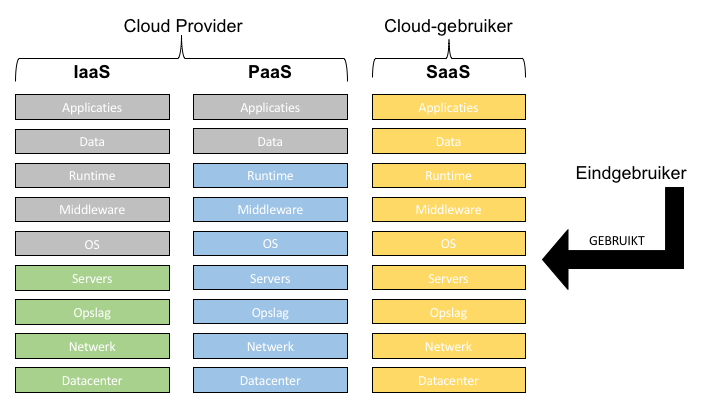
\includegraphics[scale=0.47]{cloud_rollen}
		}
	\end{subfigure}
	\caption{Cloud stakeholders met de bijhorende cloud-vorm}
	\label{fig:cloud_rollen}
\end{figure}

\subsection*{titel literatuurstudie}
\addcontentsline{toc}{subsection}{titel literatuurstudie}  
Vul aan
\chapter{Achtergrond}
\label{chap:rel_work}

Dit hoofdstuk bevat een overzicht van belangrijke achtergrondinformatie die doorheen de rest van deze scriptie gebruikt wordt. We starten met de overgang van GPUs van een hulpmiddel voor grafisch intensieve toepassingen naar een \textit{general purpose framework} waarin ze momenteel vaak gebruikt worden. Daarnaast zien we hoe een \textit{high level} programmeertaal zoals Julia aan de hand van een \textit{GPU package} abstracties kan invoeren om de efficiëntie van een programmeur te verbeteren. 

\section{General purpose GPU}
\label{sec:related_work}

Om aan hedendaagse computationele vereisten te voldoen, zoeken hard- en softwareontwikkelaars naar oplossingen via gespecialiseerde processoren. Zogenaamde \textit{hardware accelerators} zijn geoptimaliseerd voor specifieke taken (in het geval van GPUs, parallelle verwerking) en hebben voor die taken een betere performantie dan sequentiële processoren die voldoen aan meer generieke vereisten \cite{Besard_2019}. GPUs zijn origineel ontwikkeld om het \textit{rendering} proces van afbeeldingen en 3D scènes (voor onder andere videospellen) te versnellen. De nodige berekeningen zijn van nature \textit{floating-point} intensief en de grote \textit{throughput} door de parallelle verwerking maken GPUs interessant voor niet grafische toepassingen \cite{Springer2013}. 

\subsection{General purpose programming frameworks}
\label{subsec:gpp_frameworks}

Oude hardware was moeilijk te programmeren voor niet grafische taken. De vaste \textit{graphics pipelines} moesten met een specifieke \textit{application programming interfaces (API)} aangestuurd worden. Zo ontstonden twee belangrijke en \textit{vendor} onafhankelijke APIs, Microsoft's DirectX \cite{MicrosoftDX2018} en Silicon Graphics' OpenGL \cite{OpenGL2021}. Wanneer men via deze APIs een niet grafische toepassing wou programmeren, dan moest het probleem eerst omgezet worden naar een equivalente schakeling van grafische operaties \cite{Springer2013}.

Deze aanpak blijkt in de praktijk niet haalbaar te zijn en leidde tot verdere innovaties. In 2006 introduceerde NVIDIA de \textit{Compute Unified Device Architecture (CUDA)}. Een API om via CUDA C (een extensie van de C programmeertaal en later C++) toegang te krijgen tot een NVIDIA GPU zijn virtuele instructieset en parallelle uitvoeringscapaciteiten \cite{NVIDIADOC2021}\cite{Adve2012}. Het geeft de nodige controle aan de programmeur om te spreken van een \textit{general purpose programming framework (GPGPU)}. Later kwamen ook de nodige uitbreidingen om dit te realiseren voor DirectX en OpenGL, verder wordt CUDA in meer detail besproken.

% Misschien beter om deze section te laten vallen en eerder te vermelden dat we enkel naar CUDA kijken.
\section{NVIDIA CUDA Toolkit}
\label{sec:nv_cuda_toolkit}

Verder wordt enkel de NVIDIA CUDA Toolkit besproken. Het is ook de focus van de realisaties in HOOFDSTUK X. De eerste hoofdstukken van de CUDA Toolkit documentatie geven een duidelijk overzicht over nieuwe concepten, interacties en hoe ze beide interageren. Het wordt dan ook als voornaamste bron gebruikt in deze sectie \cite{NVIDIADOC2021}.


\subsection{Programmeermodel}

Aanvankelijk introduceren we twee vaakgebruikte termen in het CUDA programmeermodel. \textit{Host} en \textit{device}. Met \textit{host} wordt er verwezen naar de CPU van het systeem, zo is \textit{host code} instructies die op de CPU uitgevoerd worden. De GPU noemen we het \textit{device} met gelijke analogie voor \textit{device code}. De interactie tussen de \textit{host} en het \textit{device} kan in grote lijnen als volgt weergegeven worden \cite{Gupta2020}:

\begin{itemize}
	\item[--] Host-to-device transfer: kopiëren van data uit het host geheugen naar het device geheugen.
	\item[--] Laden en uitvoeren van een device kernel (zie \nameref{subsec:programminginterface}).
	\item[--] Device-to-host transfer: kopieer het resultaat terug naar het host geheugen.
\end{itemize}

% thread hierarchy moet hier komen

% Waarom heeft elke thread in een warp zijn eigen instruction address counter als elke thread in de warp dezelfde instructie moet uitvoeren of anders gedisabled wordt? https://docs.nvidia.com/cuda/cuda-c-programming-guide/index.html#simt-architecture

De NVIDIA GPU architectuur is gebouwd rond een schaalbare reeks \textit{streaming multiprocessors (SMs)}. Wanneer de host een \textit{kernel grid} opstart, worden de verschillende blokken overlopen en threads van die blok overgedragen aan een \textit{multiprocessor} (die typisch honderden threads gelijktijdig kan uitvoeren). In realiteit worden threads in een groep van 32 toegekend, ook wel een \textit{warp} genoemd. Threads in een \textit{warp} werken volgens het \textit{Single Instruction, Multiple Thread (SIMT)} principe. Dit wilt zeggen dat elke thread hetzelfde startadres heeft (ze voeren dezelfde instructies uit) maar hebben elk een eigen \textit{instruction address counter} en \textit{register state} waardoor ze onafhankelijk van elkaar werken.

\subsection{Geheugen hierarchy}

\subsection{Programmeerinterface}
\label{subsec:programminginterface}

% SIMT architecture
% nvcc en llvm ptx backend

\begin{code}
	\inputminted{c++}{codelistings/vecadd.cu}
	\caption{Vector optelling op de GPU \cite{Harris2017}. TODO: trim code en toon enkel de relevante stukken, voor de rest verwijzen naar het artikel.}
\end{code}

\subsection{Kernel programmering}

\section{High level abstracties in Julia}
\label{sec:julia_abstractions}

\iffalse
Voorbeeld listing
\begin{table}[tbp]
	\centering
	\captionsetup{justification=centering}
	\caption[Overzicht resource-allocatieschema's]{Overzicht resource-allocatieschema's \\
		A=Algoritme, P=Protocol, F=Framework S=Simulator, C=Cloud, ILP=Integer Linair Programming, GH = Greedy Heuristic, SBP=Stochastic Bin Packing, MINLP=Particle swarm, RR=Round-Robin, SA=Simulated Annealing, SMT=Satisfiabilty Module Theory, FFD=First Fit Decreasing, MI(N)=Mixed Integer (Non-), SPLE=Software Product Line Engineering, L=Lijst, G=Graaf, B=Boom, FN=Fysieke node, Mig=Migraties, (?)=Niet vermeld}
	\label{tab:resallocschemes}
	\resizebox{\textwidth}{!}{%
	\begin{tabular}{L{4cm} l C{2cm} c c c c}
		\toprule
		Naam & Jaar & Type  & A | F | P  & Invoer & Uitvoer & Getest  \\ \midrule
		Alicherry et al.~\cite{Alicherry2012} & 2012 & k-sneden & A & G & par\{G\} & S \\
		MCRVMP~\cite{Biran2012} & 2012 & ILP \& GH & A & B\{netwerk\} & VM-plaatsing & C\\
		\bottomrule
	\end{tabular}}
\end{table}

In Tabel~\ref{tab:resallocschemes} wordt een overzicht weergegeven ...
\fi
\chapter{chapter2 titel}
\label{chap:evaluation}

vul aan

\section{sectie titel}
\label{sec:scalable_faafo}
vul aan

Voorbeeld figuur
\begin{figure}
	\centering
	\subcaptionbox{Uitvoer van Rally \label{fig:evaluation_rally1}}{%
		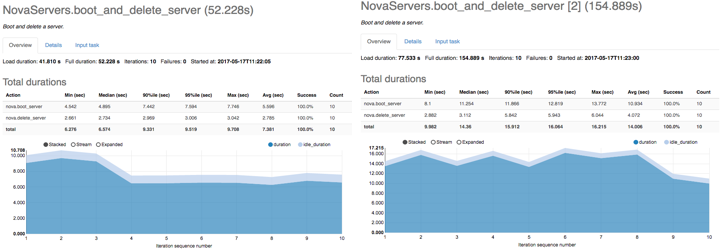
\includegraphics[width=1.00\textwidth]{Dia3}%
	}\par\medskip
	\subcaptionbox{Uitvoer van de monitorapplicatie \label{fig:evaluation_rally2}}{%
		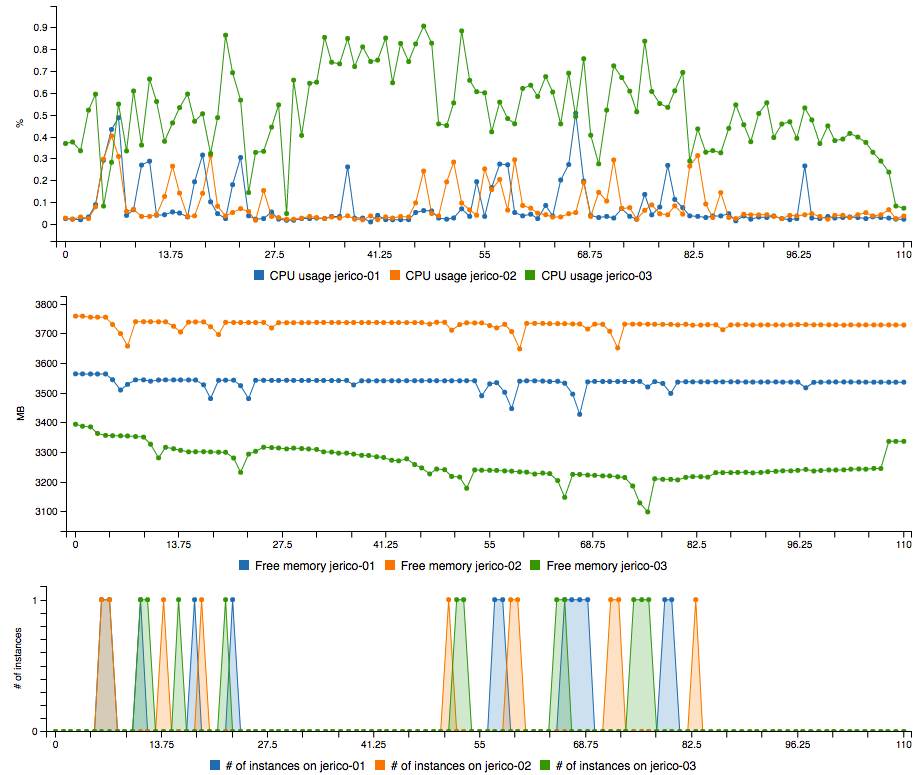
\includegraphics[width=1.00\textwidth]{rally_evaluation}%
	}
	\caption{Evaluatie met Rally - Resultaten}
	\label{fig:evaluation_rally}
\end{figure}

\chapter{chapter3 titel}


vul aan

\section{sectie titel}
vul aan

Voorbeeld listing

\subsection{code isbn}
Voorbeeld listing
\begin{code}
\inputminted{python}{isbn.py}
\caption{isbn}
\end{code}
\chapter*{Conclusie}
\addcontentsline{toc}{chapter}{Conclusie}  

vul aan

\section*{Ethische en maatschappelijke reflectie}
\addcontentsline{toc}{section}{Ethische en maatschappelijke reflectie}  
vul aan

Meer informatie kan je opzoeken op https://www.sdgs.be/nl/sdgs 
\bibliography{referenties}

\begin{appendices}
\section*{Bijlage A }
\label{att:installation}
toelichting bijlage
\end{appendices}

\end{document}
